% SMPdesign/SMPdesign.tex

\chapter{SMP Synchronization Design}
\label{cha:SMP Synchronization Design}

\QuickQuizChapter{cha:SMP Synchronization Design}

This chapter describes how to design software to take advantage of
the multiple CPUs that are increasingly appearing in commodity systems.
It does this by presenting a number of idioms, or ``design patterns''
that can help you balance performance, scalability, and realtime response.
The following section describes the ``forces'' that act on any SMP
design, namely, the desirable properties that the designer is trying
to achieve, such as good scalability, the pitfalls to be avoided,
such as contention, overhead, and complexity, and the constraints
imposed by the workload, such as read-intensity.

\section{Design Forces}
\label{sec:SMPdesign:Design Forces}

There are a number of forces that act on any programming project,
with perhaps the most (in)famous including schedule pressure, elegance,
performance, and work-life balance.
Very often, perfectly handling one of the forces acting on the
project will sacrifice the others, so that the most aggressive
possible schedule will likely involve sacrifices in the areas of
elegance, performance, and work-life balance.

A given design pattern may be thought of as a particular way
of balancing the forces acting on the design,
with particularly good idioms, or ``design patterns'', describing
particularly good balances among those forces~\cite{Alexander79,GOF95}.

The forces acting on the performance of parallel programs are
speedup,
contention, overhead, read-to-write ratio, and complexity:
\begin{description}
\item[Speedup:]  Getting a program to run faster is the
	only reason to go to all of the time and trouble
	required to parallelize it.
	Speedup is defined to be the ratio of the time required
	to run a sequential version of the program to the time
	required to run a parallel version.
\item[Contention:]  If more CPUs are applied to a parallel
	program than can be kept busy by that program,
	the excess CPUs are prevented from doing
	useful work by contention.
\item[Work-to-Synchronization Ratio:]  A uniprocessor,
	single-threaded, non-preemptible, and non-interruptible\footnote{
		Either by masking interrupts or by being oblivious to them.}
	version of a given parallel
	program would not need the synchronization primitives.
	Therefore, any time consumed by these primitives
	(including communication cache misses as well as
	locking primitives, atomic instructions, and memory
	barriers)
	is overhead that does not contribute directly to the useful
	work that the program is intended to accomplish.
	Note that the important measure is the
	relationship between the synchronization overhead
	and the overhead of the code in the critical section, with larger
	critical sections able to tolerate greater synchronization overhead.
\item[Read-to-Write Ratio:]  A data structure that is
	rarely updated may often be protected with asymmetric
	synchronization primitives that reduce readers' synchronization
	overhead at the expense of that of writers, thereby
	reducing overall synchronization overhead.
	Corresponding optimizations are possible for frequently
	updated data structures, as discussed in
	Section~\ref{sec:advsync:Simple NBS} on
	Page~\pageref{sec:advsync:Simple NBS}.
\item[Complexity:]  A parallel program is more complex than
	an equivalent sequential program because the parallel
	program has a much larger state space than does the
	sequential program.  A parallel programmer must
	consider synchronization primitives, locking design,
	critical-section identification,
	and deadlock in the context of this larger state space.

	This greater complexity often translates
	to higher development and maintenance costs.
	Therefore, budgetary constraints can
	limit the number and types of modifications made to
	an existing program, since a given degree of speedup is
	worth only so much time and trouble.
\end{description}
These forces will act together to enforce a maximum speedup.
The first three forces are deeply interrelated, so
the remainder of this section analyzes these
interrelationships.\footnote{
	A real-world parallel system will have many additional
	forces acting on it, such as data-structure layout,
	memory size, memory-hierarchy latencies, and bandwidth limitations.}

Note that these forces may also appear as part of the context.
For example, speedup may act as a force (``the faster, the better'')
or as a requirement of the workload, or ``context'' (``the system must
support at least 10,000 web hits per second'').

An understanding of the relationships between these forces can
be very helpful when resolving the forces acting on an existing
parallel program.
\begin{enumerate}
\item	The less time a program spends in critical sections,
	the greater the potential speedup.
\item	The fraction of time that the program spends in
	a given critical section must be much less than
	the reciprocal of the number of CPUs for the
	actual speedup to approach the number of CPUs.
	For example, a program running on 10 CPUs must spend
	much less than one tenth of its time in the critical section
	if it is to scale well.
\item	Contention effects will consume the excess CPU and/or
	wallclock time should the actual speedup be less than
	the number of available CPUs.  The
	larger the gap between the number of CPUs
	and the actual speedup, the less efficiently the
	CPUs will be used.
	Similarly, the greater the desired efficiency, the smaller
	the achievable speedup.
\item	If the available synchronization primitives have
	high overhead compared to the critical sections
	that they guard, the best way to improve speedup
	is to reduce the number of times that the primitives
	are invoked (perhaps by fusing critical sections,
	using data ownership, using RCU,
	or by moving toward a more coarse-grained parallelism
	such as code locking).
\item	If the critical sections have high overhead compared
	to the primitives guarding them, the best way
	to improve speedup is to increase parallelism
	by moving to reader/writer locking, data locking, RCU,
	or data ownership.
\item	If the critical sections have high overhead compared
	to the primitives guarding them and the data structure
	being guarded is read much more often than modified,
	the best way to increase parallelism is to move
	to reader/writer locking or RCU.
\item	Many changes that improve SMP performance, for example,
	reducing lock contention, also improve realtime latencies.
\end{enumerate}

\section{Lock Granularity}
\label{sec:SMPdesign:Lock Granularity}

Figure~\ref{fig:SMPdesign:Design Patterns and Lock Granularity}
gives a pictoral view of different levels of locking granularity,
each of which is described in one of the following sections.

\begin{figure}[htb]
\begin{center}
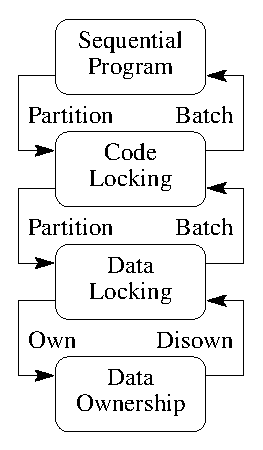
\includegraphics{SMPdesign/LockGranularity}
\end{center}
\caption{Design Patterns and Lock Granularity}
\label{fig:SMPdesign:Design Patterns and Lock Granularity}
\end{figure}

\subsection{Sequential Program}
\label{sec:SMPdesign:Sequential Program}

If the program runs fast enough on a single processor, and
has no interactions with other processes, threads, or interrupt
handlers, you should
remove the synchronization primitives and spare yourself their
overhead and complexity.
Some would argue that Moore's Law will eventually force all
programs into this category.
Others would disagree, particularly given the decrease in
% @@@ Intel Trademark
rate of CPU clock-frequency growth in Intel CPUs since the year 2003,
as can be seen in
Figure~\ref{fig:SMPdesign:Clock-Frequency Trend for Intel CPUs}.
The debate as to whether this leveling-off will result in single chips
with thousands
of CPUs will not be settled soon, but given that Paul is typing this
sentence on a dual-core laptop, the age of SMP does seem to be upon us.

\begin{figure}[htb]
\begin{center}
\resizebox{3in}{!}{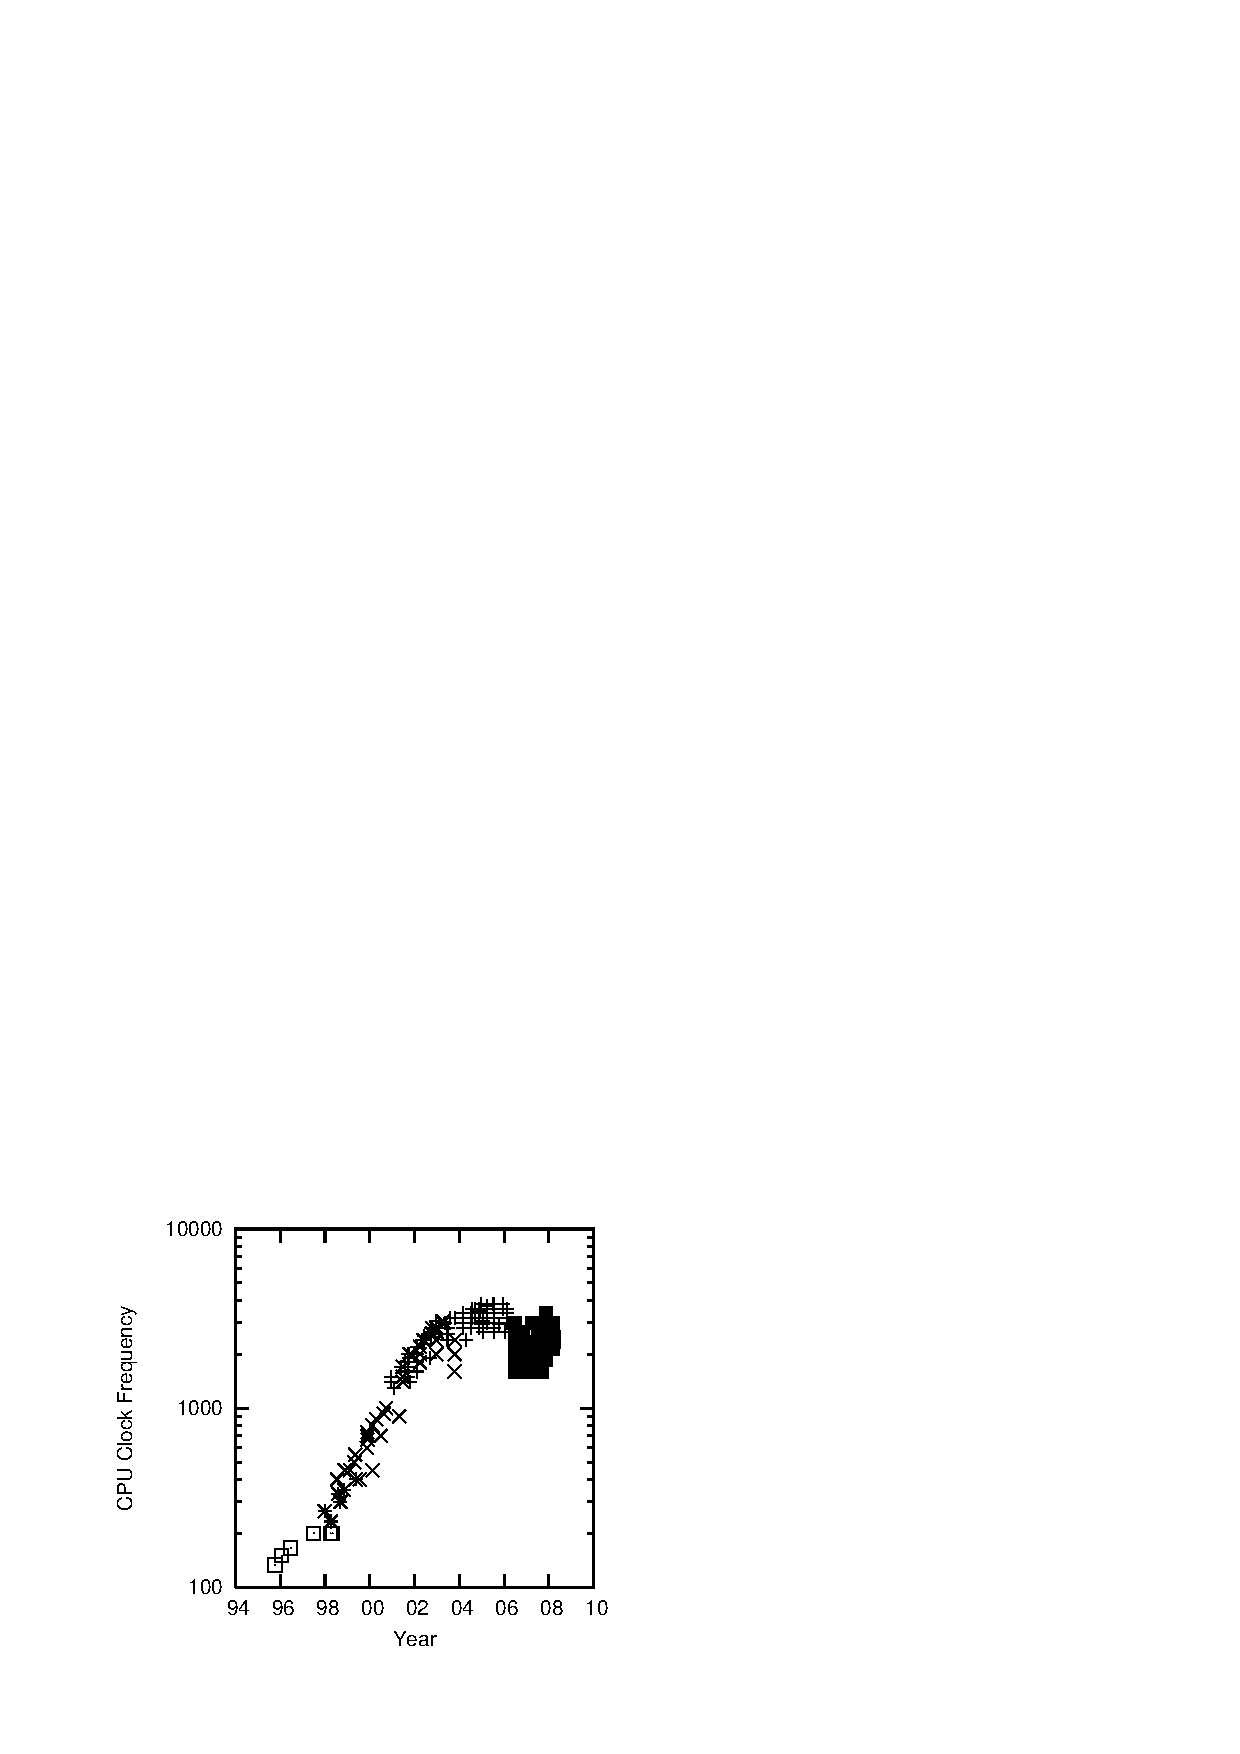
\includegraphics{SMPdesign/clockfreq}}
\end{center}
\caption{Clock-Frequency Trend for Intel CPUs}
\label{fig:SMPdesign:Clock-Frequency Trend for Intel CPUs}
\end{figure}

Please note that this does \emph{not} mean that you should code each
and every program in a multi-threaded manner.
Again, if a program runs quickly enough on a single processor,
spare yourself the overhead and complexity of SMP synchronization
primitives.
The simplicity of the hash-table lookup code in
Figure~\ref{fig:SMPdesign:Sequential-Program Hash Table Search}
underscores this point.\footnote{
	The examples in this section are taken from Hart et
	al.~\cite{ThomasEHart2006a}, adapted for clarity
	by gathering code related code from multiple files.}

\begin{figure}[htbp] 
{ \scriptsize
\begin{verbatim}
  1 struct hash_table
  2 {
  3   long nbuckets;
  4   struct node **buckets;
  5 };
  6 
  7 typedef struct node {
  8   unsigned long key;
  9   struct node *next;
 10 } node_t;
 11 
 12 int hash_search(struct hash_table *h, long key)
 13 {
 14   struct node *cur;
 15 
 16   cur = h->buckets[key % h->nbuckets];
 17   while (cur != NULL) {
 18     if (cur->key >= key) {
 19       return (cur->key == key);
 20     }
 21     cur = cur->next;
 22   }
 23   return 0;
 24 }
\end{verbatim}
}
\caption{Sequential-Program Hash Table Search}
\label{fig:SMPdesign:Sequential-Program Hash Table Search}
\end{figure}

% ./test_hash_null.exe 1000 0/100 1 1024 1
% ./test_hash_null.exe: nmilli: 1000 update/total: 0/100 nelements: 1 nbuckets: 1024 nthreads: 1
% ./test_hash_null.exe: avg = 96.2913  max = 98.2337  min = 90.4095  std = 2.95314
% ./test_hash_null.exe: nmilli: 1000 update/total: 0/100 nelements: 1 nbuckets: 1024 nthreads: 1
% ./test_hash_null.exe: avg = 91.5592  max = 97.3315  min = 89.9885  std = 2.88925
% ./test_hash_null.exe: nmilli: 1000 update/total: 0/100 nelements: 1 nbuckets: 1024 nthreads: 1
% ./test_hash_null.exe: avg = 93.3568  max = 106.162  min = 89.8828  std = 6.40418

On the other hand, if you are not in this happy situation, read on!

\subsection{Code Locking}
\label{sec:SMPdesign:Code Locking}

Code locking is the simplest locking design, using only
global locks.\footnote{
	If your program instead has locks in data structures,
	or, in the case of Java, uses classes with synchronized
	instances, you are instead using ``data locking'', described
	in Section~\ref{sec:SMPdesign:Data Locking}.}
It is especially
easy to retrofit an existing program to use code locking in
order to run it on a multiprocessor.  If the program has
only a single shared resource, code locking will even give
optimal performance.
However, many of the larger and more complex programs
require much of the execution to
occur in critical sections, which in turn causes code locking
to sharply limits their scalability.

Therefore, you should use code locking on programs that spend
only a small fraction of their execution time in critical sections or
from which only modest scaling is required.  In these cases,
code locking will provide a relatively simple program that is
very similar to its sequential counterpart,
as can be seen in
Figure~\ref{fig:SMPdesign:Code-Locking Hash Table Search}.
However, not that the simple return of the comparison in
\url{hash_search()} in
Figure~\ref{fig:SMPdesign:Sequential-Program Hash Table Search}
has now become three statements due to the need to release the
lock before returning.

\begin{figure}[htbp] 
{ \scriptsize
\begin{verbatim}
  1 spinlock_t hash_lock;
  2 
  3 struct hash_table
  4 {
  5   long nbuckets;
  6   struct node **buckets;
  7 };
  8 
  9 typedef struct node {
 10   unsigned long key;
 11   struct node *next;
 12 } node_t;
 13 
 14 int hash_search(struct hash_table *h, long key)
 15 {
 16   struct node *cur;
 17   int retval;
 18 
 19   spin_lock(&hash_lock);
 20   cur = h->buckets[key % h->nbuckets];
 21   while (cur != NULL) {
 22     if (cur->key >= key) {
 23       retval = (cur->key == key);
 24       spin_unlock(&hash_lock);
 25       return retval;
 26     }
 27     cur = cur->next;
 28   }
 29   spin_unlock(&hash_lock);
 30   return 0;
 31 }
\end{verbatim}
}
\caption{Code-Locking Hash Table Search}
\label{fig:SMPdesign:Code-Locking Hash Table Search}
\end{figure}

However, code locking is particularly prone to ``lock contention'',
where multiple CPUs need to acquire the lock concurrently.
SMP programmers who have taken care of groups of small children
(or of older people who are acting like children) will immediately
recognize the danger of having only one of something,
as illustrated in Figure~\ref{fig:SMPdesign:Lock Contention}.

% ./test_hash_codelock.exe 1000 0/100 1 1024 1
% ./test_hash_codelock.exe: nmilli: 1000 update/total: 0/100 nelements: 1 nbuckets: 1024 nthreads: 1
% ./test_hash_codelock.exe: avg = 164.115  max = 170.388  min = 161.659  std = 3.21857
% ./test_hash_codelock.exe: nmilli: 1000 update/total: 0/100 nelements: 1 nbuckets: 1024 nthreads: 1
% ./test_hash_codelock.exe: avg = 181.17  max = 198.4  min = 162.459  std = 15.8585
% ./test_hash_codelock.exe: nmilli: 1000 update/total: 0/100 nelements: 1 nbuckets: 1024 nthreads: 1
% ./test_hash_codelock.exe: avg = 167.651  max = 189.014  min = 162.144  std = 10.6819

% ./test_hash_codelock.exe 1000 0/100 1 1024 2
% ./test_hash_codelock.exe: nmilli: 1000 update/total: 0/100 nelements: 1 nbuckets: 1024 nthreads: 2
% ./test_hash_codelock.exe: avg = 378.481  max = 385.971  min = 374.235  std = 4.05934
% ./test_hash_codelock.exe: nmilli: 1000 update/total: 0/100 nelements: 1 nbuckets: 1024 nthreads: 2
% ./test_hash_codelock.exe: avg = 753.414  max = 1015.28  min = 377.734  std = 294.942
% ./test_hash_codelock.exe: nmilli: 1000 update/total: 0/100 nelements: 1 nbuckets: 1024 nthreads: 2
% ./test_hash_codelock.exe: avg = 502.737  max = 980.924  min = 374.406  std = 239.383

One solution to this problem, named ``data locking'', is described
in the next section.

\begin{figure}[htb]
\begin{center}
\resizebox{3in}{!}{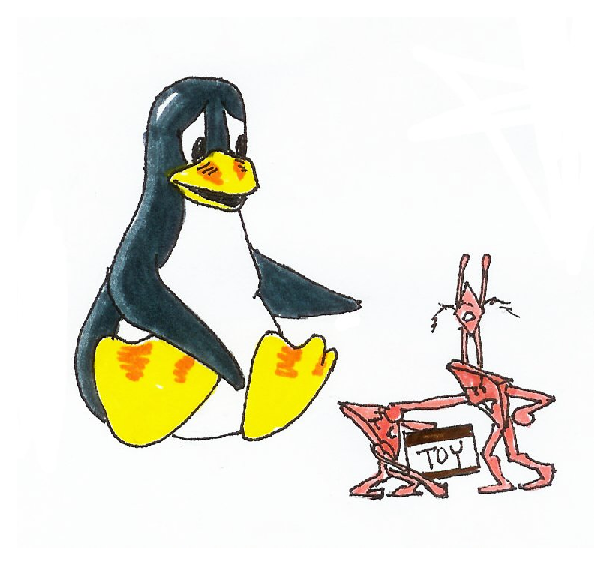
\includegraphics{cartoons/OneFighting}}
\end{center}
\caption{Lock Contention}
\label{fig:SMPdesign:Lock Contention}
\end{figure}

\subsection{Data Locking}
\label{sec:SMPdesign:Data Locking}

Many data structures may be partitioned,
with each partition of the data structure having its own lock.
Then the critical sections for each part of the data structure
can execute in parallel,
although only one instance of the critical section for a given
part could be executing at a given time.
Use data locking when contention must
be reduced, and where synchronization overhead is not
limiting speedups.
Data locking reduces contention by distributing the instances
of the overly-large critical section into multiple critical sections,
for example, maintaining per-hash-bucket critical sections in a
hash table, as shown in
Figure~\ref{fig:SMPdesign:Data-Locking Hash Table Search}.
The increased scalability again results in increased complexity
in the form of an additional data structure, the \url{struct bucket}.

\begin{figure}[htbp] 
{ \scriptsize
\begin{verbatim}
  1 struct hash_table
  2 {
  3   long nbuckets;
  4   struct bucket **buckets;
  5 };
  6 
  7 struct bucket {
  8   spinlock_t bucket_lock;
  9   node_t *list_head;
 10 };
 11 
 12 typedef struct node {
 13   unsigned long key;
 14   struct node *next;
 15 } node_t;
 16 
 17 int hash_search(struct hash_table *h, long key)
 18 {
 19   struct bucket *bp;
 20   struct node *cur;
 21   int retval;
 22 
 23   bp = h->buckets[key % h->nbuckets];
 24   spin_lock(&bp->bucket_lock);
 25   cur = bp->list_head;
 26   while (cur != NULL) {
 27     if (cur->key >= key) {
 28       retval = (cur->key == key);
 29       spin_unlock(&bp->hash_lock);
 30       return retval;
 31     }
 32     cur = cur->next;
 33   }
 34   spin_unlock(&bp->hash_lock);
 35   return 0;
 36 }
\end{verbatim}
}
\caption{Data-Locking Hash Table Search}
\label{fig:SMPdesign:Data-Locking Hash Table Search}
\end{figure}

In contrast with the contentious situation
shown in Figure~\ref{fig:SMPdesign:Lock Contention},
data locking helps promote harmony, as illustrated by
Figure~\ref{fig:SMPdesign:Data Locking} --- and in parallel programs,
this \emph{almost} always translates into increased performance and
scalability.
For this reason, data locking was heavily used by Sequent in
both its DYNIX and DYNIX/ptx operating
systems~\cite{Beck85,Inman85,Garg90,Dove90,McKenney92b,McKenney92a,McKenney93}.

\begin{figure}[htb]
\begin{center}
\resizebox{3in}{!}{\includegraphics{cartoons/ManyHappy}}
\end{center}
\caption{Data Locking}
\label{fig:SMPdesign:Data Locking}
\end{figure}

% ./test_hash_spinlock.exe 1000 0/100 1 1024 1
% ./test_hash_spinlock.exe: nmilli: 1000 update/total: 0/100 nelements: 1 nbuckets: 1024 nthreads: 1
% ./test_hash_spinlock.exe: avg = 158.118  max = 162.404  min = 156.199  std = 2.19391
% ./test_hash_spinlock.exe: nmilli: 1000 update/total: 0/100 nelements: 1 nbuckets: 1024 nthreads: 1
% ./test_hash_spinlock.exe: avg = 157.717  max = 162.446  min = 156.415  std = 2.36662
% ./test_hash_spinlock.exe: nmilli: 1000 update/total: 0/100 nelements: 1 nbuckets: 1024 nthreads: 1
% ./test_hash_spinlock.exe: avg = 158.369  max = 164.75  min = 156.501  std = 3.19454

% ./test_hash_spinlock.exe 1000 0/100 1 1024 2
% ./test_hash_spinlock.exe: nmilli: 1000 update/total: 0/100 nelements: 1 nbuckets: 1024 nthreads: 2
% ./test_hash_spinlock.exe: avg = 223.426  max = 422.948  min = 167.858  std = 100.136
% ./test_hash_spinlock.exe: nmilli: 1000 update/total: 0/100 nelements: 1 nbuckets: 1024 nthreads: 2
% ./test_hash_spinlock.exe: avg = 235.462  max = 507.134  min = 167.466  std = 135.836
% ./test_hash_spinlock.exe: nmilli: 1000 update/total: 0/100 nelements: 1 nbuckets: 1024 nthreads: 2
% ./test_hash_spinlock.exe: avg = 305.807  max = 481.685  min = 167.939  std = 132.589

However, as those how have taken care of small children can again attest,
even providing enough to go around is no guarantee of tranquillity.
The analogous situation can arise in SMP programs.
For example, the Linux kernel maintains a cache of files and directories
(called ``dcache'').
Each entry in this cache has its own lock, but the entries corresponding
to the root directory and its direct descendants are much more likely to
be traversed than are more obscure entries.
This can result in many CPUs contending for the locks of these popular
entries, resulting in a situation not unlike that
shown in Figure~\ref{fig:SMPdesign:Data and Skew}.

\begin{figure}[htb]
\begin{center}
\resizebox{3in}{!}{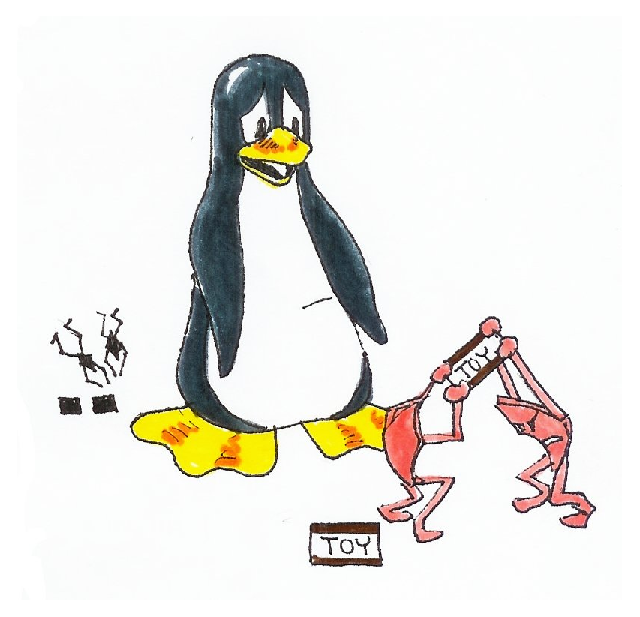
\includegraphics{cartoons/ManyFighting}}
\end{center}
\caption{Data Locking and Skew}
\label{fig:SMPdesign:Data and Skew}
\end{figure}

In many cases, algorithms can be designed to reduce the instance of
data skew, and in some cases eliminate it entirely
(as appears to be possible with the Linux kernel's dcache~\cite{McKenney04a}).
Data locking is often used for partitionable data structures such as
hash tables, as well as in situations where multiple entities are each
represented by an instance of a given data structure.
The task list in version 2.6.17 of the Linux kernel is an example of the
latter, each task structure having its own \url{proc_lock}.

\subsection{Data Ownership}
\label{sec:SMPdesign:Data Ownership}

Data ownership partitions a given data structure over the threads
or CPUs, so that each thread/CPU accesses its subset of the data
structure without any synchronization overhead whatsoever.
However, if one thread wishes to access some other thread's data,
the first thread is unable to do so directly.
Instead, the first thread must communicate with the second thread,
so that the second thread performs the operation on behalf of the
first, or, alternatively, migrates the data to the first thread.

Data ownership might seem arcane, but it is used very frequently:
\begin{enumerate}
\item	Any variables accessible by only one CPU or thread
	(such as {\tt auto} variables in C
	and C++) are owned by that CPU or process.
\item	An instance of a user interface owns the corresponding
	user's context.  It is very common for applications
	interacting with parallel database engines to be
	written as if they were entirely sequential programs.
	Such applications own the user interface and his current
	action.  Explicit parallelism is thus confined to the
	database engine itself.
\item	Parametric simulations are often trivially parallelized
	by granting each thread ownership of a particular region
	of the parameter space.
\end{enumerate}

If there is significant sharing, communication between the threads
or CPUs can result in significant complexity and overhead.
Furthermore, if the most-heavily used data happens to be that owned
by a single CPU, that CPU will be a ``hot spot'', sometimes with
results resembling that shown in Figure~\ref{fig:SMPdesign:Data and Skew}.
However, in situations where no sharing is required, data ownership
achieves ideal performance, and with code that can be as simple
as the sequential-program case shown in
Figure~\ref{fig:SMPdesign:Sequential-Program Hash Table Search}.
Such situations are often referred to as ``embarassingly
parallel'', and, in the best case, resemble the situation
previously shown in Figure~\ref{fig:SMPdesign:Data Locking}.

% ./test_hash_null.exe 1000 0/100 1 1024 1
% ./test_hash_null.exe: nmilli: 1000 update/total: 0/100 nelements: 1 nbuckets: 1024 nthreads: 1
% ./test_hash_null.exe: avg = 96.2913  max = 98.2337  min = 90.4095  std = 2.95314
% ./test_hash_null.exe: nmilli: 1000 update/total: 0/100 nelements: 1 nbuckets: 1024 nthreads: 1
% ./test_hash_null.exe: avg = 91.5592  max = 97.3315  min = 89.9885  std = 2.88925
% ./test_hash_null.exe: nmilli: 1000 update/total: 0/100 nelements: 1 nbuckets: 1024 nthreads: 1
% ./test_hash_null.exe: avg = 93.3568  max = 106.162  min = 89.8828  std = 6.40418

% ./test_hash_null.exe 1000 0/100 1 1024 2
% ./test_hash_null.exe: nmilli: 1000 update/total: 0/100 nelements: 1 nbuckets: 1024 nthreads: 2
% ./test_hash_null.exe: avg = 45.4526  max = 46.4281  min = 45.1954  std = 0.487791
% ./test_hash_null.exe: nmilli: 1000 update/total: 0/100 nelements: 1 nbuckets: 1024 nthreads: 2
% ./test_hash_null.exe: avg = 46.0238  max = 49.2861  min = 45.1852  std = 1.63127
% ./test_hash_null.exe: nmilli: 1000 update/total: 0/100 nelements: 1 nbuckets: 1024 nthreads: 2
% ./test_hash_null.exe: avg = 46.6858  max = 52.6278  min = 45.1761  std = 2.97102

Another important instance of data ownership occurs when the data
is read-only.
If nobody will change the data, everyone can own it.
In SMP design, only constant data ``wants to be free''.
Data that is subject to change requires some sort of access control.\footnote{
	That said, please understand that the authors are in no way
	advocating for copyright, trademark, or patent rights for CPUs!}

\subsection{Locking Granularity and Performance}
\label{sec:SMPdesign:Locking Granularity and Performance}

\emph{@@@ summarize performance and scalability here, once
we get clean performance numbers.}

\section{Parallel Fastpath}
\label{sec:SMPdesign:Parallel Fastpath}

Fine-grained (and therefore \emph{usually} higher-performance)
designs are typically more complex than are coarser-grained designs.
In many cases, most of the overhead is incurred by a small fraction
of the code~\cite{Knuth73}.
So why not focus effort on that small fraction?

This is the idea behind the parallel-fastpath design pattern, to aggressively
parallelize the common-case code path without incurring the complexity
that would be required to aggressively parallelize the entire algorithm.
You must understand not only the specific algorithm you wish
to parallelize, but also the workload that the algorithm will
be subjected to.  Great creativity and design
effort is often required to construct a parallel fastpath.

Parallel fastpath combines different patterns (one for the 
fastpath, one elsewhere) and is therefore a template pattern.
The following instances of parallel
fastpath occur often enough to warrant their own patterns,
as depicted in Figure~\ref{fig:SMPdesign:Parallel-Fastpath Design Patterns}:

\begin{figure}[htb]
\begin{center}
% \resizebox{3in}{!}{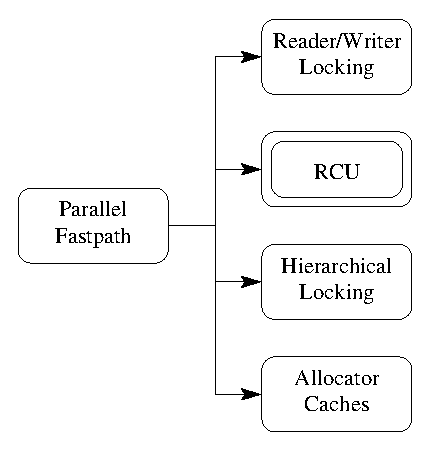
\includegraphics{SMPdesign/ParallelFastpath}}
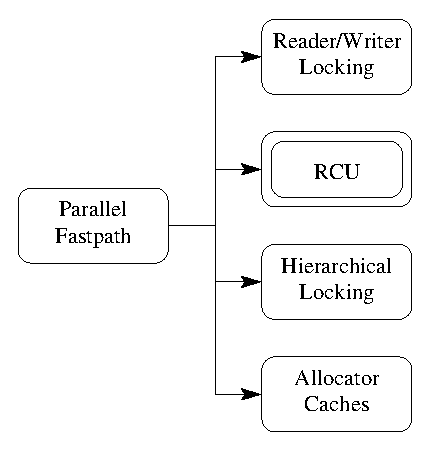
\includegraphics{SMPdesign/ParallelFastpath}
\end{center}
\caption{Parallel-Fastpath Design Patterns}
\label{fig:SMPdesign:Parallel-Fastpath Design Patterns}
\end{figure}

\begin{enumerate}
\item	Reader/Writer Locking
	(described below in Section~\ref{sec:SMPdesign:Reader/Writer Locking}).
\item	Read-copy update (RCU), which is very briefly described below
	in Section~\ref{sec:defer:Read-Copy Update (RCU)}).
\item   Hierarchical Locking~(\cite{McKenney95b}).
\item	Resource Allocator Caches~(\cite{McKenney95b,McKenney93}).
	See Chapter~\ref{chp:Memory Allocation} for more detail.
\end{enumerate}

\subsection{Reader/Writer Locking}
\label{sec:SMPdesign:Reader/Writer Locking}

If synchronization overhead is negligible (for example, if the program
uses coarse-grained parallelism), and if only a small fraction of the
critical sections modify data, then allowing multiple readers
to proceed in parallel can greatly increase scalability.
Writers exclude both readers and each other.
Figure~\ref{fig:SMPdesign:Reader-Writer-Locking Hash Table Search}
shows how the hash search might be implemented using reader-writer locking.

\begin{figure}[htbp] 
{ \scriptsize
\begin{verbatim}
  1 rwlock_t hash_lock;
  2 
  3 struct hash_table
  4 {
  5   long nbuckets;
  6   struct node **buckets;
  7 };
  8 
  9 typedef struct node {
 10   unsigned long key;
 11   struct node *next;
 12 } node_t;
 13 
 14 int hash_search(struct hash_table *h, long key)
 15 {
 16   struct node *cur;
 17   int retval;
 18 
 19   read_lock(&hash_lock);
 20   cur = h->buckets[key % h->nbuckets];
 21   while (cur != NULL) {
 22     if (cur->key >= key) {
 23       retval = (cur->key == key);
 24       read_unlock(&hash_lock);
 25       return retval;
 26     }
 27     cur = cur->next;
 28   }
 29   read_unlock(&hash_lock);
 30   return 0;
 31 }
\end{verbatim}
}
\caption{Reader-Writer-Locking Hash Table Search}
\label{fig:SMPdesign:Reader-Writer-Locking Hash Table Search}
\end{figure}

Reader/writer locking is a simple instance of asymmetric locking.
Snaman~\cite{Snaman87} describes a more ornate six-mode
asymmetric locking design used in several clustered systems.
Asymmetric locking primitives can be used to implement a very
simple form of the {\bf Observer Pattern}~\cite{GOF95}--when a
writer releases the lock, all readers are notified of the change
in state.

\subsection{Read-Copy Update Introduction}
\label{sec:SMPdesign:Read-Copy Update Introduction}

Read-copy update (RCU) is a mutual-exclusion mechanism which can be
used as an alternative to reader-writer locking.
RCU features extremely low-overhead wait-free read-side critical sections,
however, updates can be expensive, as they must leave old versions of the
data structure in place for the sake of pre-existing readers.
These old versions may be reclaimed once all such pre-existing readers
complete their accesses.~\cite{WikipediaRCU}.

It turns out that our example hash-search program is well-suited to RCU.
Other programs may be more difficult to adapt to RCU,
and more detail on such adaptation may be found in
Section~\ref{sec:defer:Read-Copy Update (RCU)}.

In some implementations of RCU
(such as that of Hart et al.~\cite{ThomasEHart2006a}),
the search code can be implemented
exactly as in sequential programs, as was shown in
Figure~\ref{fig:SMPdesign:Sequential-Program Hash Table Search}.
However, other environments, including the Linux kernel, require
that the RCU read-side critical sections be marked explicitly,
as shown in
Figure~\ref{fig:SMPdesign:RCU Hash Table Search}.
Such marking can be a great favor to whoever must later read the code!

\begin{figure}[htbp] 
{ \scriptsize
\begin{verbatim}
  1 struct hash_table
  2 {
  3   long nbuckets;
  4   struct node **buckets;
  5 };
  6 
  7 typedef struct node {
  8   unsigned long key;
  9   struct node *next;
 10 } node_t;
 11 
 12 int hash_search(struct hash_table *h, long key)
 13 {
 14   struct node *cur;
 15   int retval;
 16 
 17   rcu_read_lock();
 18   cur = h->buckets[key % h->nbuckets];
 19   while (cur != NULL) {
 20     if (cur->key >= key) {
 21       retval = (cur->key == key);
 22       rcu_read_unlock();
 23       return retval;
 24     }
 25     cur = cur->next;
 26   }
 27   rcu_read_unlock();
 28   return 0;
 29 }
\end{verbatim}
}
\caption{RCU Hash Table Search}
\label{fig:SMPdesign:RCU Hash Table Search}
\end{figure}

Update-side code must wait for a ``grace period'' after removing an
element before freeing it, and RCU implementations provide special
primitives for this purpose.
For example, the Linux kernel provides \url{synchronize_rcu()} to
block until the end of a subsequent grace period (and other related primitives
as well),
while Hart et al.~\cite{ThomasEHart2006a} provide a \url{free_node_later()}
primitive that frees the specified data element after the end of a
subsequent grace period (in contrast to their \url{free_node()} primitive
that immediately frees the specified data element).

RCU's greatest strength is its low-overhead (in some cases, zero-overhead)
read-side primitives.
In many implementations, these primitives are in fact deterministic,
which is useful in realtime environments.

\subsection{Hierarchical Locking}
\label{sec:SMPdesign:Hierarchical Locking}

The idea behind hierarchical locking is to have a coarse-grained lock
that is held only long enough to work out which fine-grained lock
to acquire.
Figure~\ref{fig:SMPdesign:Hierarchical-Locking Hash Table Search}
shows how our hash-table search might be adapted to do hierarchical
locking, but also shows the great weakness of this approach:
we have paid the overhead of acquiring a second lock, but we only
hold it for a short time.
In this case, the simpler data-locking approach would be simpler
and likely perform better.

\begin{figure}[htbp] 
{ \scriptsize
\begin{verbatim}
  1 struct hash_table
  2 {
  3   long nbuckets;
  4   struct bucket **buckets;
  5 };
  6 
  7 struct bucket {
  8   spinlock_t bucket_lock;
  9   node_t *list_head;
 10 };
 11 
 12 typedef struct node {
 13   spinlock_t node_lock;
 14   unsigned long key;
 15   struct node *next;
 16 } node_t;
 17 
 18 int hash_search(struct hash_table *h, long key)
 19 {
 20   struct bucket *bp;
 21   struct node *cur;
 22   int retval;
 23 
 24   bp = h->buckets[key % h->nbuckets];
 25   spin_lock(&bp->bucket_lock);
 26   cur = bp->list_head;
 27   while (cur != NULL) {
 28     if (cur->key >= key) {
 29       spin_lock(&cur->node_lock);
 30       spin_unlock(&bp->bucket_lock);
 31       retval = (cur->key == key);
 32       spin_unlock(&cur->node_lock);
 33       return retval;
 34     }
 35     cur = cur->next;
 36   }
 37   spin_unlock(&bp->bucket_lock);
 38   return 0;
 39 }
\end{verbatim}
}
\caption{Hierarchical-Locking Hash Table Search}
\label{fig:SMPdesign:Hierarchical-Locking Hash Table Search}
\end{figure}

\QuickQuiz{}
	In what situation would hierarchical locking work well?
\QuickQuizAnswer{
	If the comparison on line~31 of
	Figure~\ref{fig:SMPdesign:Hierarchical-Locking Hash Table Search}
	were replaced by a much heavier-weight operation,
	then releasing {\tt bp->bucket\_lock} \emph{might} reduce lock
	contention enough to outweigh the overhead of the extra
	acquisition and release of {\tt cur->node\_lock}.
} \QuickQuizEnd

\subsection{Resource Allocator Caches}
\label{sec:SMPdesign:Resource Allocator Caches}

This section presents a simplified schematic of a parallel fixed-block-size
memory allocator.
More detailed descriptions may be found in the
literature~\cite{McKenney92a,McKenney93,Bonwick01slab,McKenney01e}
or in the Linux kernel~\cite{Torvalds2.6kernel}.

\subsubsection{Parallel Resource Allocation Problem}

The basic problem facing a parallel memory allocator is the tension
between the need to provide extremely fast memory allocation and
freeing in the common case and the need to efficiently distribute
memory in face of unfavorable allocation and freeing patterns.

To see this tension, consider a straightforward application of
data ownership to this problem --- simply carve up memory so that
each CPU owns its share.
For example, suppose that a system with two CPUs has two gigabytes
of memory (such as the one that I am typing on right now).
We could simply assign each CPU one gigabyte of memory, and allow
each CPU to access its own private chunk of memory, without the
need for locking and its complexities and overheads.
Unfortunately, this simple scheme breaks down if an algorithm happens
to have CPU 0 allocate all of the memory and CPU 1 the free it, as
would happen in a simple producer-consumer workload.

The other extreme, code locking, suffers from excessive lock contention
and overhead~\cite{McKenney93}.

\subsubsection{Parallel Fastpath for Resource Allocation}

The commonly used solution uses parallel fastpath with each CPU
owning a modest cache of blocks, and with a large code-locked
shared pool for additional blocks.
To prevent any given CPU from monopolizing the memory blocks,
we place a limit on the number of blocks that can be in each CPU's
cache.
In a two-CPU system, the flow of memory blocks will be as shown
in Figure~\ref{fig:SMPdesign:Allocator Cache Schematic}:
when a given CPU is trying to free a block when its pool is full,
it sends blocks to the global pool, and, similarly, when that CPU
is trying to allocate a block when its pool is empty, it retrieves
blocks from the global pool.

\begin{figure}[htb]
\begin{center}
\resizebox{3in}{!}{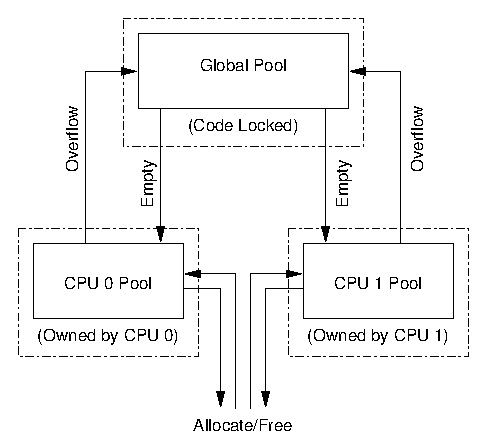
\includegraphics{SMPdesign/allocatorcache}}
\end{center}
\caption{Allocator Cache Schematic}
\label{fig:SMPdesign:Allocator Cache Schematic}
\end{figure}

\subsubsection{Data Structures}

The actual data structures for a ``toy'' implementation of allocator
caches are shown in
Figure~\ref{fig:SMPdesign:Allocator-Cache Data Structures}.
The ``Global Pool'' of Figure~\ref{fig:SMPdesign:Allocator Cache Schematic}
is implemented by \url{globalmem} of type \url{struct globalmempool},
and the two CPU pools by the per-CPU variable \url{percpumem} of
type \url{percpumempool}.
Both of these data structures have arrays of pointers to blocks
in their \url{pool} fields, which are filled from index zero upwards.
Thus, if \url{globalmem.pool[3]} is \url{NULL}, then the remainder of
the array from index 4 up must also be NULL.
The \url{cur} fields contain the index of the highest-numbered full
element of the \url{pool} array, or -1 if all elements are empty.
All elements from \url{globalmem.pool[0]} through
\url{globalmem.pool[globalmem.cur]} must be full, and all the rest
must be empty.\footnote{
	Both pool sizes (\url{TARGET_POOL_SIZE} and
	\url{GLOBAL_POOL_SIZE}) are unrealistically small, but this small
	size makes it easier to single-step the program in order to get
	a feel for its operation.}

\begin{figure}[htbp] 
{ \scriptsize
\begin{verbatim}
  1 #define TARGET_POOL_SIZE 3
  2 #define GLOBAL_POOL_SIZE 40
  3 
  4 struct globalmempool {
  5   spinlock_t mutex;
  6   int cur;
  7   struct memblock *pool[GLOBAL_POOL_SIZE];
  8 } globalmem;
  9 
 10 struct percpumempool {
 11   int cur;
 12   struct memblock *pool[2 * TARGET_POOL_SIZE];
 13 };
 14 
 15 DEFINE_PER_THREAD(struct percpumempool, percpumem);
\end{verbatim}
}
\caption{Allocator-Cache Data Structures}
\label{fig:SMPdesign:Allocator-Cache Data Structures}
\end{figure}

The operation of the pool data structures is illustrated by
Figure~\ref{fig:SMPdesign:Allocator Pool Schematic},
with the six boxes representing the array of pointers making up
the \url{pool} field, and the number preceding them representing
the \url{cur} field.
The shaded boxes represent non-\url{NULL} pointers, while the empty
boxes represent \url{NULL} pointers.
An important, though potentially confusing, invariant of this
data structure is that the \url{cur} field is always one
smaller than the number of non-\url{NULL} pointers.

\begin{figure}[htb]
\begin{center}
\resizebox{3in}{!}{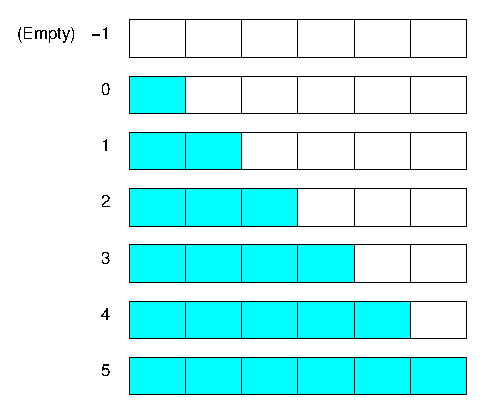
\includegraphics{SMPdesign/AllocatorPool}}
\end{center}
\caption{Allocator Pool Schematic}
\label{fig:SMPdesign:Allocator Pool Schematic}
\end{figure}

\subsubsection{Allocation Function}

The allocation function \url{memblock_alloc()} may be seen in
Figure~\ref{fig:SMPdesign:Allocator-Cache Allocator Function}.
Line~7 picks up the current thread's per-thread pool,
and line~8 check to see if it is empty.

If so, lines~9-16 attempt to refill it from the global pool
under the spinlock acquired on line~9 and released on line~16.
Lines~10-14 move blocks from the global to the per-thread pool until
either the local pool reaches its target size (half full) or
the global pool is exhausted, and line~15 sets the per-thread pool's
count to the proper value.

In either case, line~18 checks for the per-thread pool still being
empty, and if not, lines~19-21 remove a block and return it.
Otherwise, line~23 tells the sad tale of memory exhaustion.

\begin{figure}[htbp] 
{ \scriptsize
\begin{verbatim}
  1 struct memblock *memblock_alloc(void)
  2 {
  3   int i;
  4   struct memblock *p;
  5   struct percpumempool *pcpp;
  6
  7   pcpp = &__get_thread_var(percpumem);
  8   if (pcpp->cur < 0) {
  9     spin_lock(&globalmem.mutex);
 10     for (i = 0; i < TARGET_POOL_SIZE &&
 11                 globalmem.cur >= 0; i++) {
 12       pcpp->pool[i] = globalmem.pool[globalmem.cur];
 13       globalmem.pool[globalmem.cur--] = NULL;
 14     }
 15     pcpp->cur = i - 1;
 16     spin_unlock(&globalmem.mutex);
 17   }
 18   if (pcpp->cur >= 0) {
 19     p = pcpp->pool[pcpp->cur];
 20     pcpp->pool[pcpp->cur--] = NULL;
 21     return p;
 22   }
 23   return NULL;
 24 }
\end{verbatim}
}
\caption{Allocator-Cache Allocator Function}
\label{fig:SMPdesign:Allocator-Cache Allocator Function}
\end{figure}

\subsubsection{Free Function}

Figure~\ref{fig:SMPdesign:Allocator-Cache Free Function} shows
the memory-block free function.
Line~6 gets a pointer to this thread's pool, and
line~7 checks to see if this per-thread pool is full.

If so, lines~8-15 empty half of the per-thread pool into the global pool,
with lines~8 and 14 acquiring and releasing the spinlock.
Lines~9-12 implement the loop moving blocks from the local to the
global pool, and line~13 sets the per-thread pool's count to the proper
value.

In either case, line~16 then places the newly freed block into the
per-thread pool.

\begin{figure}[htbp] 
{ \scriptsize
\begin{verbatim}
  1 void memblock_free(struct memblock *p)
  2 {
  3   int i;
  4   struct percpumempool *pcpp;
  5 
  6   pcpp = &__get_thread_var(percpumem);
  7   if (pcpp->cur >= 2 * TARGET_POOL_SIZE - 1) {
  8     spin_lock(&globalmem.mutex);
  9     for (i = pcpp->cur; i >= TARGET_POOL_SIZE; i--) {
 10       globalmem.pool[++globalmem.cur] = pcpp->pool[i];
 11       pcpp->pool[i] = NULL;
 12     }
 13     pcpp->cur = i;
 14     spin_unlock(&globalmem.mutex);
 15   }
 16   pcpp->pool[++pcpp->cur] = p;
 17 }
\end{verbatim}
}
\caption{Allocator-Cache Free Function}
\label{fig:SMPdesign:Allocator-Cache Free Function}
\end{figure}

\subsubsection{Performance}

Rough performance results\footnote{
	This data was not collected in a statistically meaningful way,
	and therefore should be viewed with great skepticism and suspicion.
	Good data-collection and -reduction practice is discussed
	in Chapter @@@.
	That said, repeated runs gave similar results, and these results
	match more careful evaluations of similar algorithms.}
are shown in
Figure~\ref{fig:SMPdesign:Allocator Cache Performance},
running on a dual-core Intel x86 running at 1GHz (4300 bogomips per CPU)
with at most six blocks allowed in each CPU's cache.
In this micro-benchmark,
each thread repeated allocates a group of blocks and then frees it, with
the size of the group being the ``allocation run length'' displayed on
the x-axis.
The y-axis shows the number of successful allocation/free pairs per
microsecond --- failed allocations are not counted.
The ``X''s are from a two-thread run, while the ``+''s are from a
single-threaded run.

\begin{figure}[htb]
\begin{center}
\resizebox{3in}{!}{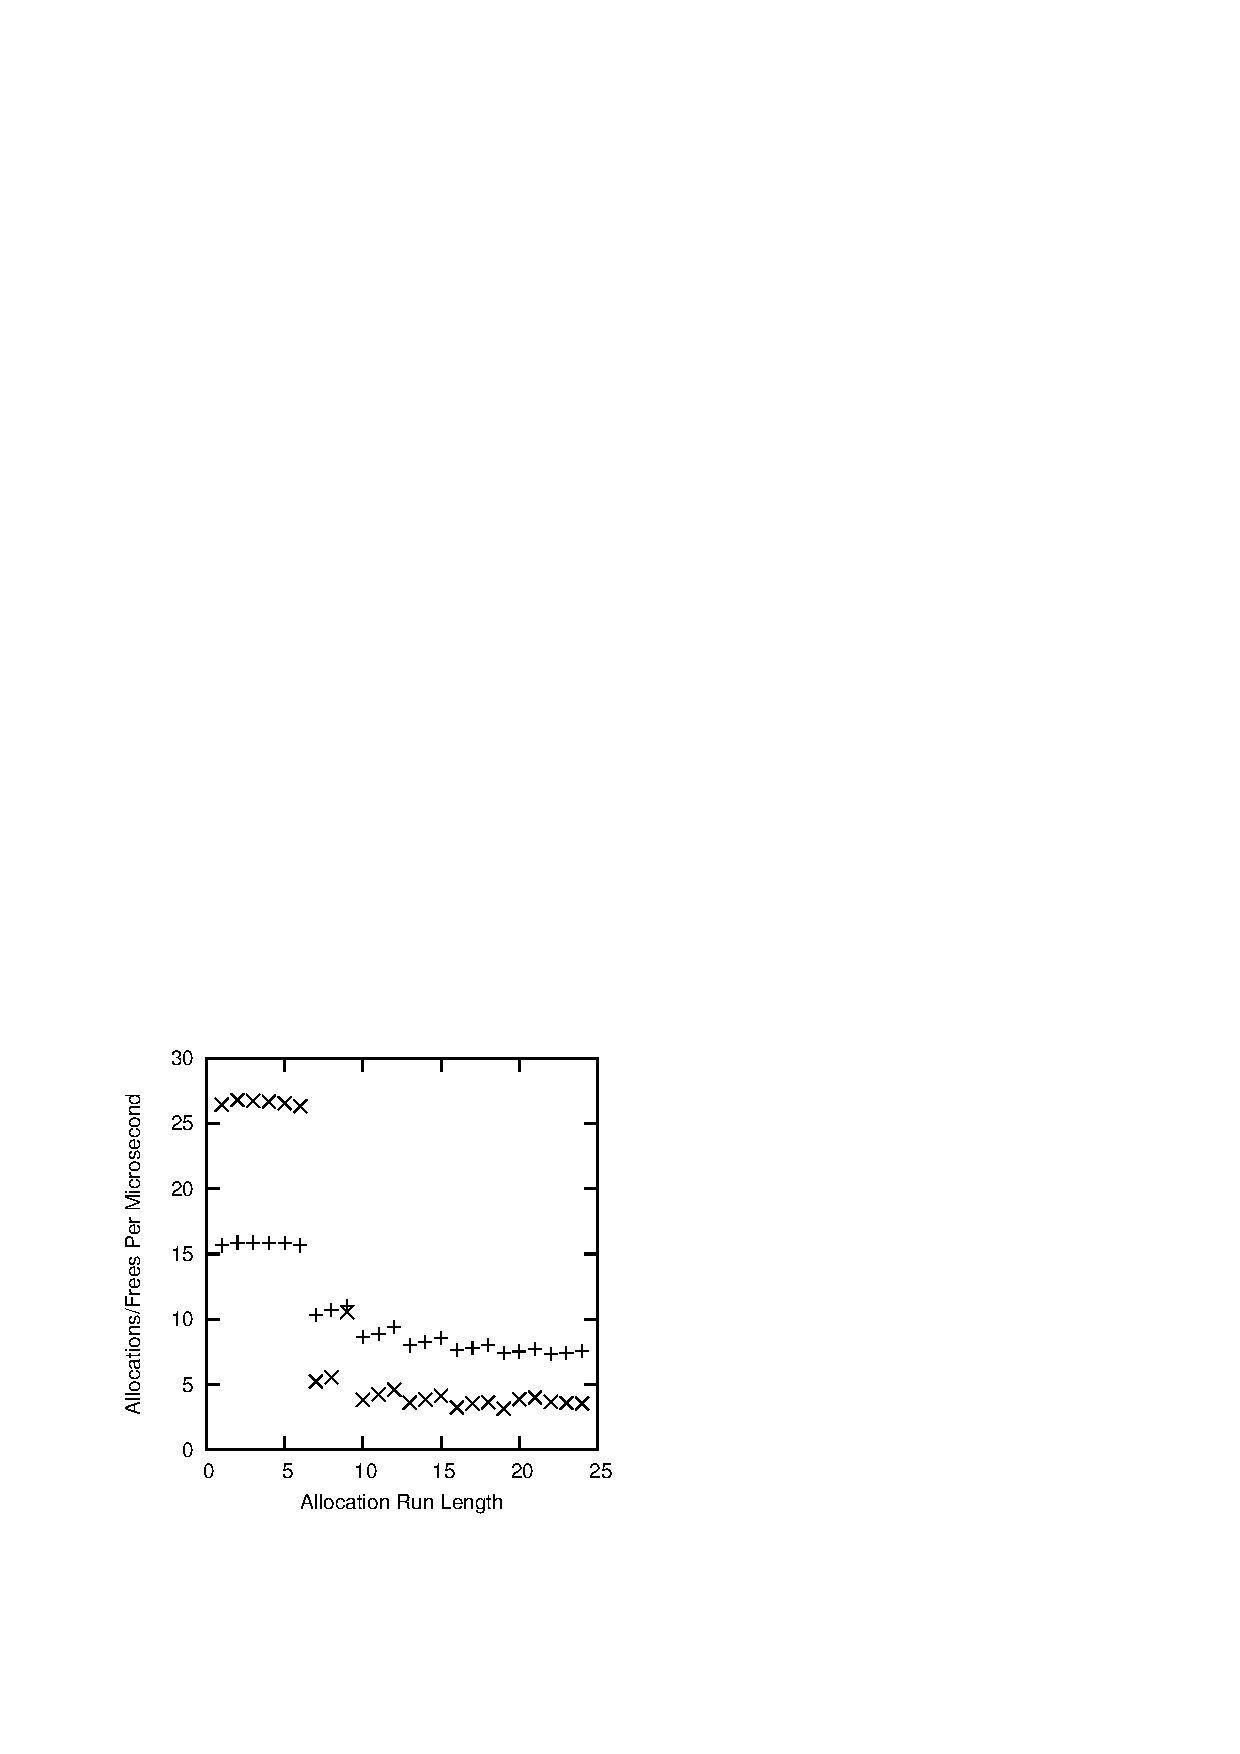
\includegraphics{SMPdesign/smpalloc}}
\end{center}
\caption{Allocator Cache Performance}
\label{fig:SMPdesign:Allocator Cache Performance}
\end{figure}

Note that run lengths up to six scale linearly and give excellent performance,
while run lengths greater than six show poor performance and almost always
also show \emph{negative} scaling.
It is therefore quite important to size \url{TARGET_POOL_SIZE}
sufficiently large,
which fortunately is usually quite easy to do in actual
practice~\cite{McKenney01e}, especially given today's large memories.
For example, in most systems, it is quite reasonable to set
\url{TARGET_POOL_SIZE} to 100, in which case allocations and frees
are guaranteed to be confined to per-thread pools at least 99\% of
the time.

As can be seen from the figure, the situations where the common-case
data-ownership applies (run lengths up to six) provide greatly improved
performance compared to the cases where locks must be acquired.
Avoiding locking in the common case will be a recurring theme through
this book.

\QuickQuiz{}
	In Figure~\ref{fig:SMPdesign:Allocator Cache Performance},
	there is a pattern of performance rising with increasing run
	length in groups of three samples, for example, for run lengths
	10, 11, and 12.
	Why?
\QuickQuizAnswer{
	This is due to the per-CPU target value being three.
	A run length of 12 must acquire the global-pool lock twice,
	while a run length of 13 must acquire the global-pool lock
	three times.
} \QuickQuizEnd

\QuickQuiz{}
	Allocation failures were observed in the two-thread
	tests at run lengths of 19 and greater.
	Given the global-pool size of 40 and the per-CPU target
	pool size of three, what is the smallest allocation run
	length at which failures can occur?
\QuickQuizAnswer{
	The exact solution to this problem is left as an exercise to
	the reader.
	The first solution received will be credited to its submitter.
	As a rough rule of thumb, the global pool size should be at least
	$m+2sn$, where
	``m'' is the maximum number of elements allocated at a given time,
	``s'' is the per-CPU pool size,
	and ``n'' is the number of CPUs.
} \QuickQuizEnd

\subsubsection{Real-World Design}

The toy parallel resource allocator was quite simple, but real-world
designs expand on this approach in a number of ways.

First, real-world allocators are required to handle a wide range
of allocation sizes, as opposed to the single size shown in this
toy example.
One popular way to do this is to offer a fixed set of sizes, spaced
so as to balance external and internal fragmentation, such as in
the late-1980s BSD memory allocator~\cite{McKusick88}.
Doing this would mean that the ``globalmem'' variable would need
to be replicated on a per-size basis, and that the associated
lock would similarly be replicated, resulting in data locking
rather than the toy program's code locking.

Second, production-quality systems must be able to repurpose memory,
meaning that they must be able to coalesce blocks into larger structures,
such as pages~\cite{McKenney93}.
This coalescing will also need to be protected by a lock, which again
could be replicated on a per-size basis.

Third, coalesced memory must be returned to the underlying memory
system, and pages of memory must also be allocated from the underlying
memory system.
The locking required at this level will depend on that of the underlying
memory system, but could well be code locking.
Code locking can often be tolerated at this level, because this
level is so infrequently reached in well-designed systems~\cite{McKenney01e}.

Despite this real-world design's greater complexity, the underlying
idea is the same --- repeated application of parallel fastpath,
as shown in
Table~\ref{fig:app:questions:Schematic of Real-World Parallel Allocator}.

\begin{table}[htbp]
{ \scriptsize
\begin{tabular}{l|l|p{1in}}
Level	& Locking & Purpose \\
\hline
Per-thread pool	  & Data ownership & High-speed allocation \\
Global block pool & Data locking   & Distributing blocks among threads \\
Coalescing	  & Data locking   & Combining blocks into pages \\
System memory	  & Code locking   & Memory from/to system \\
\end{tabular}
}
\caption{Schematic of Real-World Parallel Allocator}
\label{fig:app:questions:Schematic of Real-World Parallel Allocator}
\end{table}

\section{Performance Summary}
\label{Performance Summary}

\emph{@@@ summarize performance of the various options.
Forward-reference to the RCU/NBS section.}
